Alle Berechnungen werden mit Python 3.5.1 durchgeführt.
\subsection{Auswahl der Tröpfchen\label{sec:Auswahl}}
Für jedes Elektron werden die Zeiten $t_\text{auf},t_\text{ab}$ gemittelt (siehe Tabelle \ref{fig:Zeiten}).
\begin{table}[h!]
	\centering
	\begin{tabular}{cccccc}
		& $t_0$ & $t_\text{auf}$ & $\Delta t_\text{auf}$ & $t_\text{ab}$ & $\Delta t_\text{ab}$ \\
		\hline
		Anton & 23.15 & 13.5 & 0.5  & 9.20  & 0.19  \\
Berta & 54.53 & 6.9  & 0.1  & 5.13  & 0.12  \\
Cäsar & 14.06 & 8.4  & 0.2  & 4.28  & 0.61  \\
Dora & 27.27 & 8.7  & 0.1  & 6.47  & 0.11  \\
Emil & 36.67 & 5.8  & 0.6  & 3.52  & 0.10  \\
Friedrich & 17.16 & 10.0 & 0.2  & 4.364 & 0.063 \\
Gustav & 15.60 & 3.52 & 0.08 & 2.483 & 0.080 \\
Heinrich & 25.52 & 2.39 & 0.05 & 2.027 & 0.065 \\
Ida & 18.38 & 6.0  & 0.1  & 3.384 & 0.061 \\
Julius & 24.50 & 2.77 & 0.05 & 2.026 & 0.068 \\
Kaufmann & 32.18 & 3.8  & 0.2  & 2.75  & 0.12  \\
Ludwig & 13.21 & 8.8  & 0.2  & 4.004 & 0.088 \\
Martha & 21.87 & 4.10 & 0.06 & 2.94  & 0.13  \\
Nordpol & 21.20 & 3.70 & 0.09 & 3.207 & 0.053 \\

	\end{tabular}
	\caption{Gemittelte und für die Rechnungen verwendeten Zeiten, alle Werte in \si{\second}}
	\label{fig:Zeiten}
\end{table} \\
Die während dieser Zeit zurückgelegte Strecke ist
\begin{align}
	s = \SI{2.5e-3}{\meter} \ .
\end{align}
Damit werden die Geschwindigkeiten $v_0,v_\text{auf},v_\text{ab}$ in Tabelle \ref{fig:Vel} berechnet. \\
\begin{table}[h!]
	\centering
	\begin{tabular}{cccccc|c}
		& $v_0$ & $v_\text{auf}$ & $\Delta v_\text{auf}$ & $v_\text{ab}$ & $\Delta v_\text{ab}$ & $a$ \\
		\hline
		Anton & 0.11 & 0.185 & 0.007 & 0.272 & 0.006 & 0.60  \\
Berta & 0.05 & 0.361 & 0.007 & 0.49  & 0.01  & -0.38 \\
Cäsar & 0.18 & 0.297 & 0.006 & 0.58  & 0.08  & 0.19  \\
Dora & 0.09 & 0.287 & 0.005 & 0.386 & 0.007 & 0.46  \\
Emil & 0.07 & 0.43  & 0.05  & 0.71  & 0.02  & -1.04 \\
Friedrich & 0.15 & 0.251 & 0.005 & 0.573 & 0.008 & -0.10 \\
Gustav & 0.16 & 0.71  & 0.02  & 1.01  & 0.03  & 0.07  \\
Heinrich & 0.10 & 1.04  & 0.02  & 1.23  & 0.04  & 0.03  \\
Ida & 0.14 & 0.415 & 0.007 & 0.74  & 0.01  & -0.19 \\
Julius & 0.10 & 0.90  & 0.02  & 1.23  & 0.04  & -0.62 \\
Kaufmann & 0.08 & 0.65  & 0.04  & 0.91  & 0.04  & -0.65 \\
Ludwig & 0.19 & 0.283 & 0.006 & 0.62  & 0.01  & 0.10  \\
Martha & 0.11 & 0.610 & 0.009 & 0.85  & 0.04  & -0.06 \\
Nordpol & 0.12 & 0.68  & 0.02  & 0.78  & 0.01  & 0.56  \\

	\end{tabular}
	\caption{Geschwindigkeiten der Elektronen in \SI{e-3}{\meter\per\second} und Abweichung $a$}
	\label{fig:Vel}
\end{table} \\
Um die Richtigkeit der nachfolgenden Rechnungen zu gewährleisten wird Gleichung \eqref{eq:Bedingung} überprüft. Dafür wird
\begin{align}
	v_{0,\text{exp}} = \frac{1}{2}(v_\text{ab}-v_\text{auf})
\end{align}
berechnet und die Abweichung
\begin{align}
	a = \frac{v_0-v_{0,\text{exp}}}{v_0}
\end{align}
bestimmt (siehe Tabelle \ref{fig:Vel}).

Die Elektronen, für die gilt
\begin{align}
	|a|\leq 0.5 \ ,
\end{align}
können zur weiteren Auswertung verwendet werden. Daher werden Anton, Emil, Julius, Kaufmann und Nordpol nicht mehr berücksichtigt.
\clearpage


\subsection{Berechnung der Gesamtladung}
Für die Berechnung der Ladungen \eqref{eq:ladung} bzw. der Radien \eqref{eq:radius} werden verschiedene Größen gebraucht. Sie sind in Tabelle \ref{fig:Konstanten} aufgetragen. 
Die Spannungen werden direkt gemessen und ergeben zusammen mit dem Kondensator-Durchmesser $d$ die, für die Ladung benötigte, Feldstärke
\begin{align}
	E = \frac{U}{d} \ .
\end{align}
Die Viskosität wird mit Hilfe der gemessenen Widerstände und Abbildung \ref{abb:Wid} bestimmt. Zunächst werden die Widerstände mit der Thermistor-Tabelle \ref{tab:Therm} in Temperaturen \glqq übersetzt\grqq. Damit kann dann die Viskosität aus dem Diagramm abgelesen werden. Um Ablesefehler zu minimieren wird eine Geradengleichung durch die beiden gut lesbaren Punkte $(17,1.82),(32,1.88)$ gelegt, mit der die Viskosität ausgerechnet wird:
\begin{align}
\eta_\text{L} = \SI{4.7e-8}{\newton\second\per\meter\squared\per\celsius}
(T-\SI{273.15}{\celsius}) + \SI{1.7e-5}{\newton\second\per\meter\squared}
 \ .
\end{align}
\begin{table}[h!]
	\centering
\begin{tabular}{ccccc}
	& $U$ in \si{\volt} & $T$ in \si{\kelvin} & $\eta_\text{L}$ in \SI{e-6}{\pascal\second} \\
	\hline
	\begin{center}
\begin{table}[h]
\begin{tabular}{c | c | c | c | c}
	& lin. Ausdehnungs- & Kompressions- & Molvolumen & Molmasse \\
	& koeffizient & modul & & \\
	& in \SI{e-6}{\per\kelvin} & in \SI{e+9}{\newton\per\metre\squared} & in \si{\cubic\metre\per\mol} & in \si{\gram\per\mol} \\
	\hline
	Blei & 29.0 & 42 & \SI{1.826e-05}{} & 207.2 \\
	Graphit & 8 & 33 & \SI{5.357e-06}{} & 12.0
\end{tabular}
\caption{Benötigte Konstanten\tablefootnote{aus Versuchsanleitung zu V201, Anfängerpraktikum TU Dortmund}}
\label{Konstanten}
\end{table}
\end{center}
\end{tabular}
\caption{Viskosität von Luft $\eta_\text{L}$, am Kondensator angelegte Spannungen $U$}
\label{fig:Konstanten}
\end{table}
\begin{figure}[h!]
\centering
	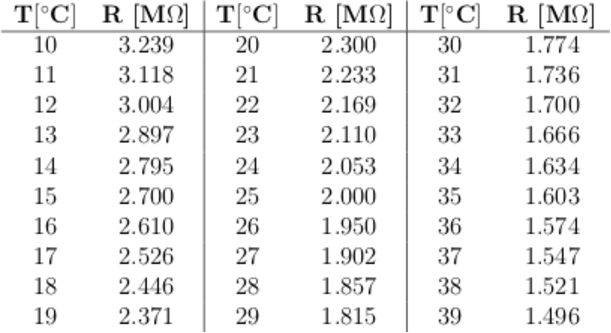
\includegraphics[width=0.55\textwidth]{Termister.pdf}
	\caption{Thermistor-Widerstandstabelle \cite{\V}}
	\label{tab:Therm}
\end{figure}
\begin{figure}[h!]
\centering
	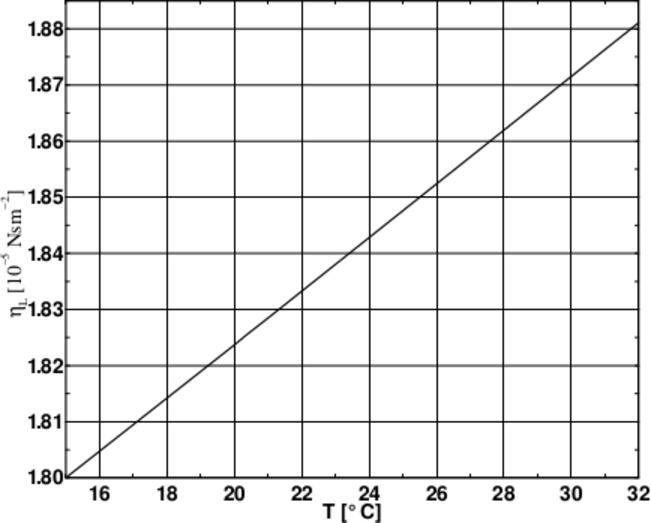
\includegraphics[width=0.6\textwidth]{Diagramm.pdf}
	\caption{Viskosität der Luft als Funktion der Temperatur \cite{\V}}
	\label{abb:Wid}
\end{figure} \\
%Die Dichte der Luft wird, unter Verwendung der allgemeinen Gasgleichung, mit
%\begin{align}
%	\rho_\text{L} = \frac{m_\text{L}}{V_\text{L}} = \frac{p}{R_\text{S}T}
%\end{align}
%berechnet. $R_\text{S} = \SI{287.058}{}$ ist die spezifische Gaskonstante für trockene Luft, $p=\SI{101325}{\pascal}$ ist der Normaldruck und $T$ die jeweilige Temperatur in Kelvin.
Eingesetzt in die Gleichungen \eqref{eq:radius} und \eqref{eq:ladung} kann so der Radius und die Ladung jedes Öltröpfchens berechnet werden (siehe Tabelle \ref{fig:RQ_unkorr}).
\begin{table}[h!]
\centering
\begin{tabular}{ccccc}
	& $r$ in \si{\micro\meter} & $\Delta r$ in \si{\micro\meter} & $q$ in \SI{e-18}{\coulomb} & $\Delta q$ in \SI{e-18}{\coulomb} \\
	\hline
	Berta & 0.79 & 0.04 & 0.54 & 0.09 \\
Cäsar & 1.2  & 0.2  & 1.8  & 0.8  \\
Dora & 0.69 & 0.03 & 0.37 & 0.05 \\
Friedrich & 1.26 & 0.02 & 1.96 & 0.09 \\
Gustav & 1.21 & 0.07 & 1.7  & 0.3  \\
Heinrich & 1.0  & 0.1  & 0.9  & 0.3  \\
Ida & 1.26 & 0.03 & 1.9  & 0.1  \\
Ludwig & 1.29 & 0.03 & 2.0  & 0.1  \\
Martha & 1.09 & 0.08 & 1.2  & 0.3  \\

\end{tabular}
\caption{Radius und unkorrigierte Ladung}
\label{fig:RQ_unkorr}
\end{table}
Wird nun die nötige Korrektur \eqref{eq:Korrektur} beachtet, sind die Ladungen der Öltröpfchen fertig bestimmt (siehe Tabelle \ref{fig:RQ_korr}).
\begin{table}[h!]
\centering
\begin{tabular}{ccc}
	& $q$ in \SI{e-18}{\coulomb} & $\Delta q$ in \SI{e-18}{\coulomb} \\
	\hline
	Berta & 0.62 & 0.09 \\
Cäsar & 2.0  & 0.8  \\
Dora & 0.44 & 0.05 \\
Friedrich & 2.2  & 0.1  \\
Gustav & 1.9  & 0.3  \\
Heinrich & 1.0  & 0.3  \\
Ida & 2.1  & 0.1  \\
Ludwig & 2.2  & 0.1  \\
Martha & 1.3  & 0.3  \\

\end{tabular}
\caption{Korrigierte Ladungen}
\label{fig:RQ_korr}
\end{table}
Diese Werte werden in Abbildung \ref{fig:Elementarladung} dargestellt.
\clearpage


\subsection{Bestimmung der Elementarladung}
Zur Bestimmung der Elementarladung wird der erste Wert
\begin{align}
	q_1 = q(r_\text{min}) = \SI{4.4(5)e-19}{\coulomb}
\end{align}
als fest angenommen, da sein Fehler sehr klein ist. Im ersten Schritt wird angenommen, dass $q_1=e_0$. Die dicken Hilfslinien im Plot werden mit diesem Abstand aufgetragen, sodass eine Ladung nahe der fünften Linie dem fünffachen der angenommenen Elementarladung $q_1$ entspricht. Dabei sind die Datenpunkte allerdings sehr weit von den Linien entfernt. In jedem nächsten Schritt wird angenommen, dass $q_1=ne_0$. Die Hilfslinien sind demnach $n$-Mal so nah beieinander. Jedes Mal wird optisch überprüft, ob die Daten zufriedenstellend nahe an den Linien liegen. Natürlich gilt, dass die Linien beliebig nah an die Punkte gebracht werden können, wenn $e_0$ nur klein genug gewählt wird. Da aber ein endliches $e_0$ gesucht wird, muss das größtmögliche $n$ bzw. $e_0$ gewählt werden. Bei $n=3$ ist die Nähe zwischen Daten und Linien zufriedenstellend. Dieser Plot ist in Abbildung \ref{fig:Elementarladung} zu sehen. \\
Die Elementarladung kann nun berechnet werden, indem für jeden Datenpunkt überprüft wird, welcher dicken Linie er am nächsten liegt. Die Gesamtladung des Öltröpfchens wird dann durch die Nummer dieser Linie geteilt. Werden diese Ergebnisse gemittelt ergibt sich schließlich die Elementarladung
\begin{align}\label{eq:Elementarladung}
	e_0 = \SI{1.6+-0.2e-19}{\coulomb}
 \ .
\end{align}
\begin{figure}[h!]
	\centering
	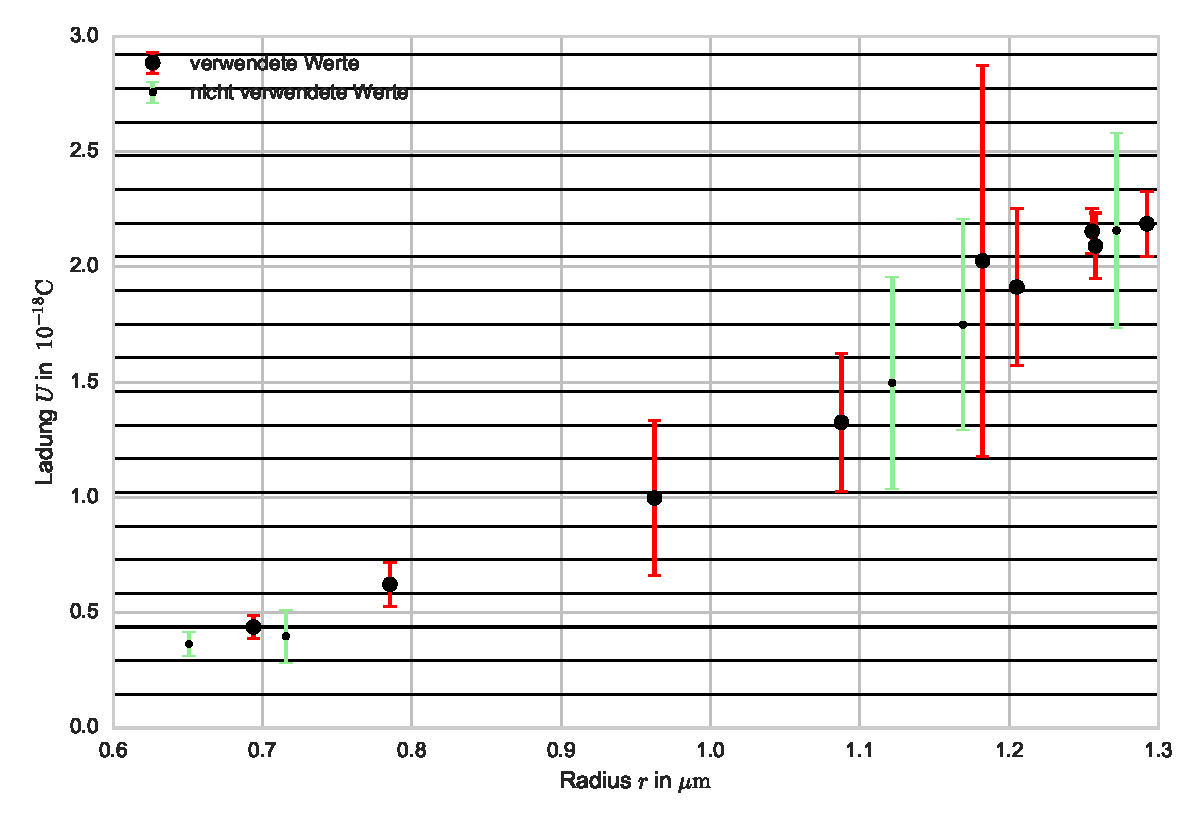
\includegraphics[width = \textwidth]{Plot.pdf}
	\caption{Zu sehen sind die Ladung der Öltröpfchen aufgetragen gegen ihren Radius. Die breiten schwarzen Hilfslinien sind das ein-, zwei-, drei-, etc. fache der vermuteten Elementarladung. Die schwachen grauen Linien sind die normalen Koordinatenlinien, die den Wert der Ladung anzeigen.}
	\label{fig:Elementarladung}
\end{figure}